\chapter{Architecture Big Data retenue}

\section{Schéma d'architecture}

\begin{figure}[h]
\centering
\resizebox{!}{0.55\textheight}{\usetikzlibrary{positioning,arrows.meta}
\begin{tikzpicture}[
  font=\small\sffamily,
  node distance=0.8cm,
  box/.style={
    rectangle, rounded corners=3pt, minimum width=3.6cm, minimum height=0.8cm,
    text centered, align=center, draw=white, very thick, text=white
  },
  rawbox/.style={box, fill=esienavy},
  procbox/.style={box, fill=esieaorange},
  storebox/.style={box, fill=esieablue},
  arrow/.style={-{Stealth[length=2.5mm]}, thick, esieagray},
  lbl/.style={font=\scriptsize\sffamily\color{esieagray}, align=center}
]
\node[storebox] (csv) {CSV brut\\ \texttt{data/raw/}};
\node[rawbox, below=of csv] (raw) {HDFS \texttt{/projet\_ia/raw}};
\node[procbox, below=of raw] (spark) {Spark\\nettoyage + transformation};
\node[rawbox, below=of spark] (proc) {HDFS \texttt{/projet\_ia/processed}};
\node[storebox, below=of proc] (hive) {Hive\\tables externes RAW + processed};
\node[procbox, below=of hive] (jupyter) {Jupyter/PySpark\\requêtes + dashboard};

\draw[arrow] (csv) -- node[lbl, right] {ingestion\\HDFS} (raw);
\draw[arrow] (raw) -- node[lbl, right] {lecture\\HDFS} (spark);
\draw[arrow] (spark) -- node[lbl, right] {écriture\\Parquet} (proc);
\draw[arrow] (proc) -- node[lbl, right] {DDL\\EXTERNAL} (hive);
\draw[arrow] (hive) -- node[lbl, right] {Hive SQL /\\Spark SQL} (jupyter);
\end{tikzpicture}
}
\caption{Flux de données de l'architecture retenue : CSV brut
  $\to$ HDFS \texttt{raw} $\to$ Spark (nettoyage/transformation)
  $\to$ HDFS \texttt{processed} $\to$ Hive (tables externes)
  $\to$ Jupyter/PySpark (requêtes et dashboard).}
\label{fig:architecture}
\end{figure}

\section{Rôle de chaque composant}

La stack est orchestrée via Docker Compose et pilotée par un unique
point d'entrée documenté.

\begin{itemize}[leftmargin=1.5em]
  \item \textbf{HDFS} (\texttt{bde2020/hadoop-namenode} /
    \texttt{hadoop-datanode}, tag \texttt{2.0.0-hadoop2.7.4-java8}) :
    stockage distribué des zones \texttt{raw} et \texttt{processed}.
  \item \textbf{Hive} (\texttt{bde2020/hive:2.3.2-postgresql-metastore})
    : metastore Thrift + HiveServer2, tables externes RAW et
    processed, requêtage SQL.
  \item \textbf{Spark} : moteur de nettoyage/transformation, exécuté en
    mode local depuis le conteneur \texttt{jupyter}
    (\texttt{jupyter/pyspark-notebook:spark-3.5.0}).
  \item \textbf{Jupyter/PySpark} : exploration interactive, requêtes
    Hive SQL/Spark SQL, dashboard.
\end{itemize}

\begin{constat}[Choix technique validé]
Choix validé avec M.~Touati~: Jupyter/PySpark remplace Zeppelin comme
interface d'analyse et de dashboard. HDFS et Hive restent le socle de
stockage et de requêtage, conformément au sujet.
\end{constat}

\begin{figure}[h]
\centering
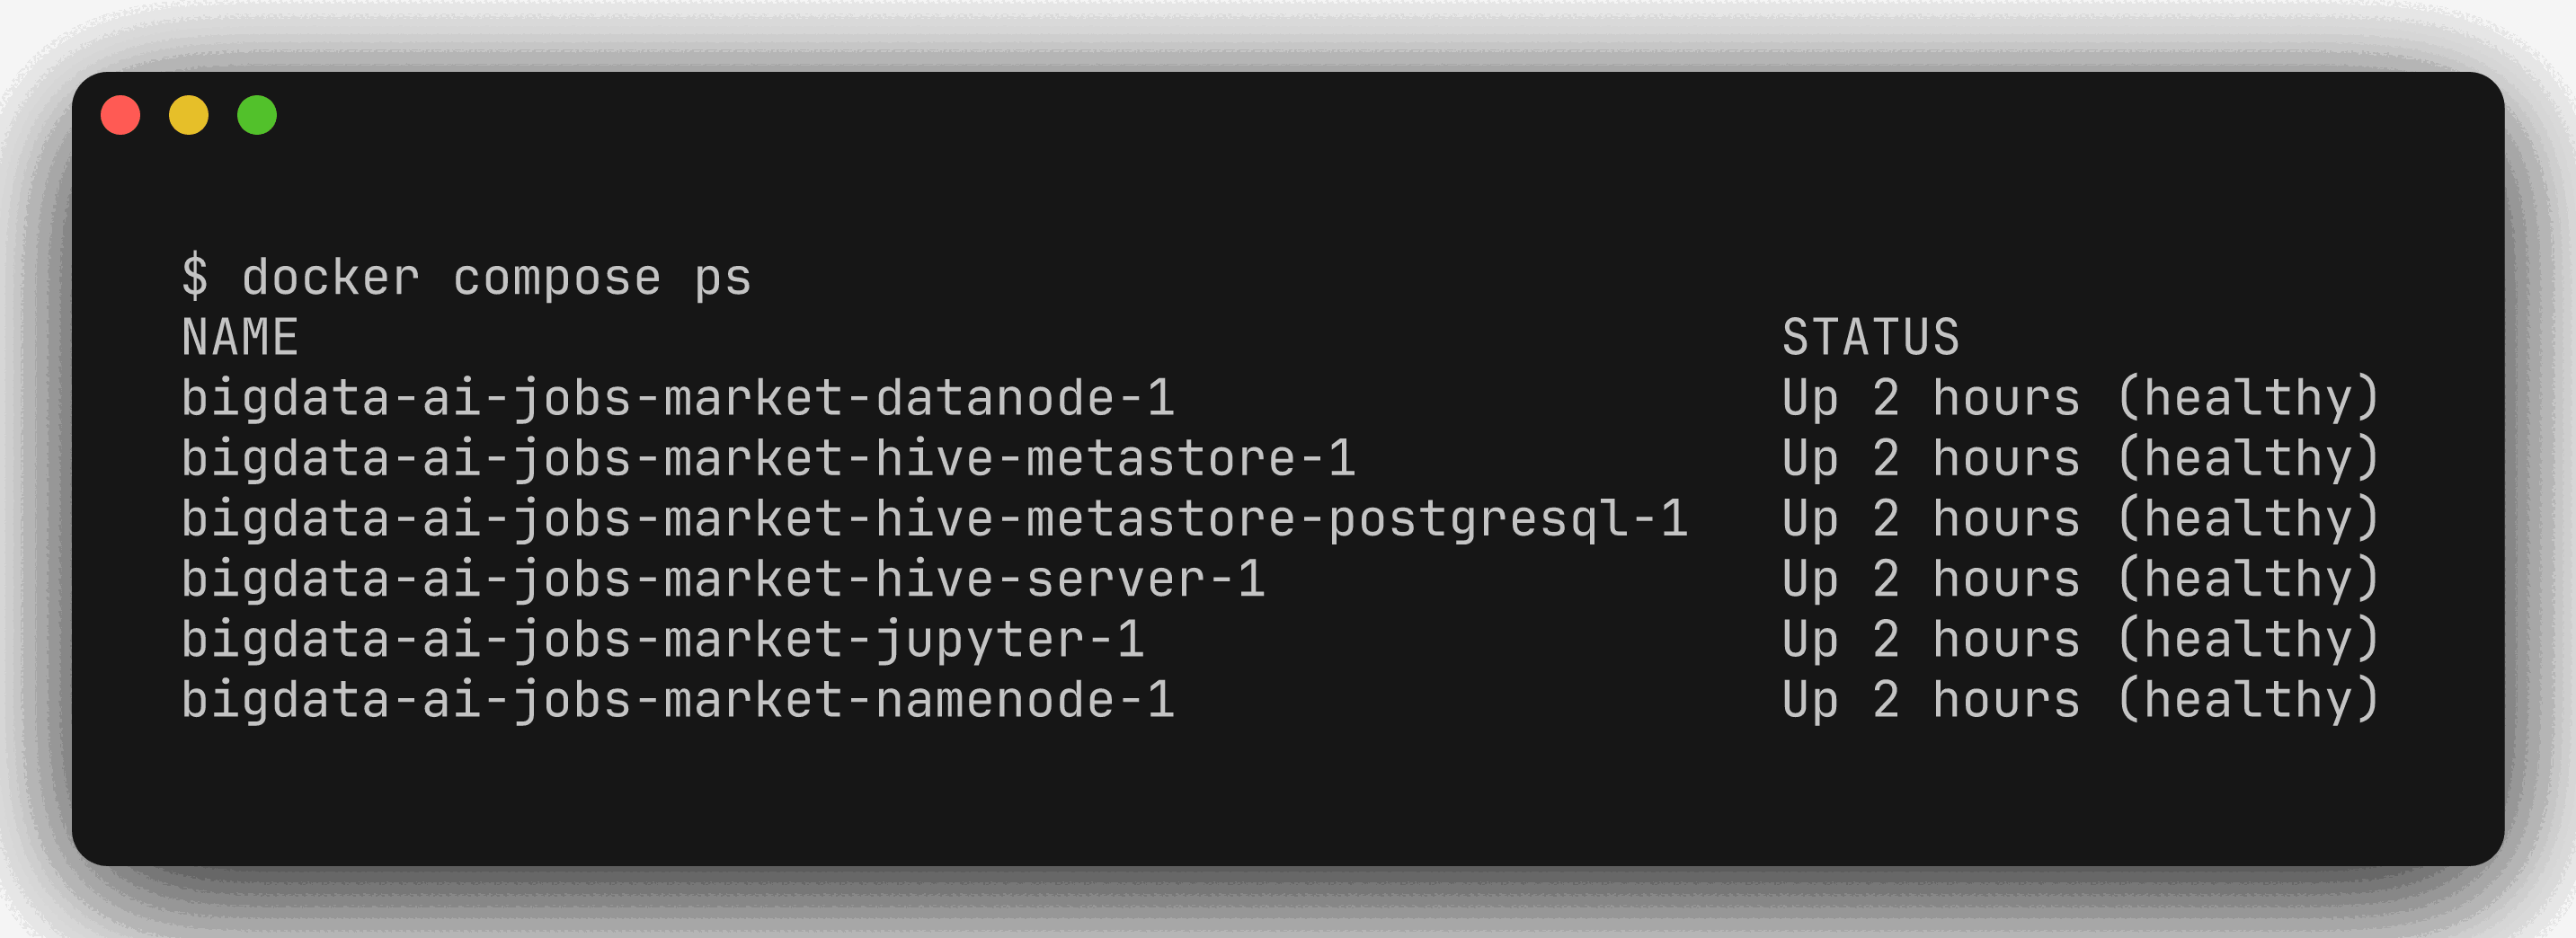
\includegraphics[width=0.85\linewidth]{figures/etape1_task_up_healthy.png}
\caption{Les 6 services de la stack Docker Compose sont healthy.}
\end{figure}

\begin{figure}[h]
\centering
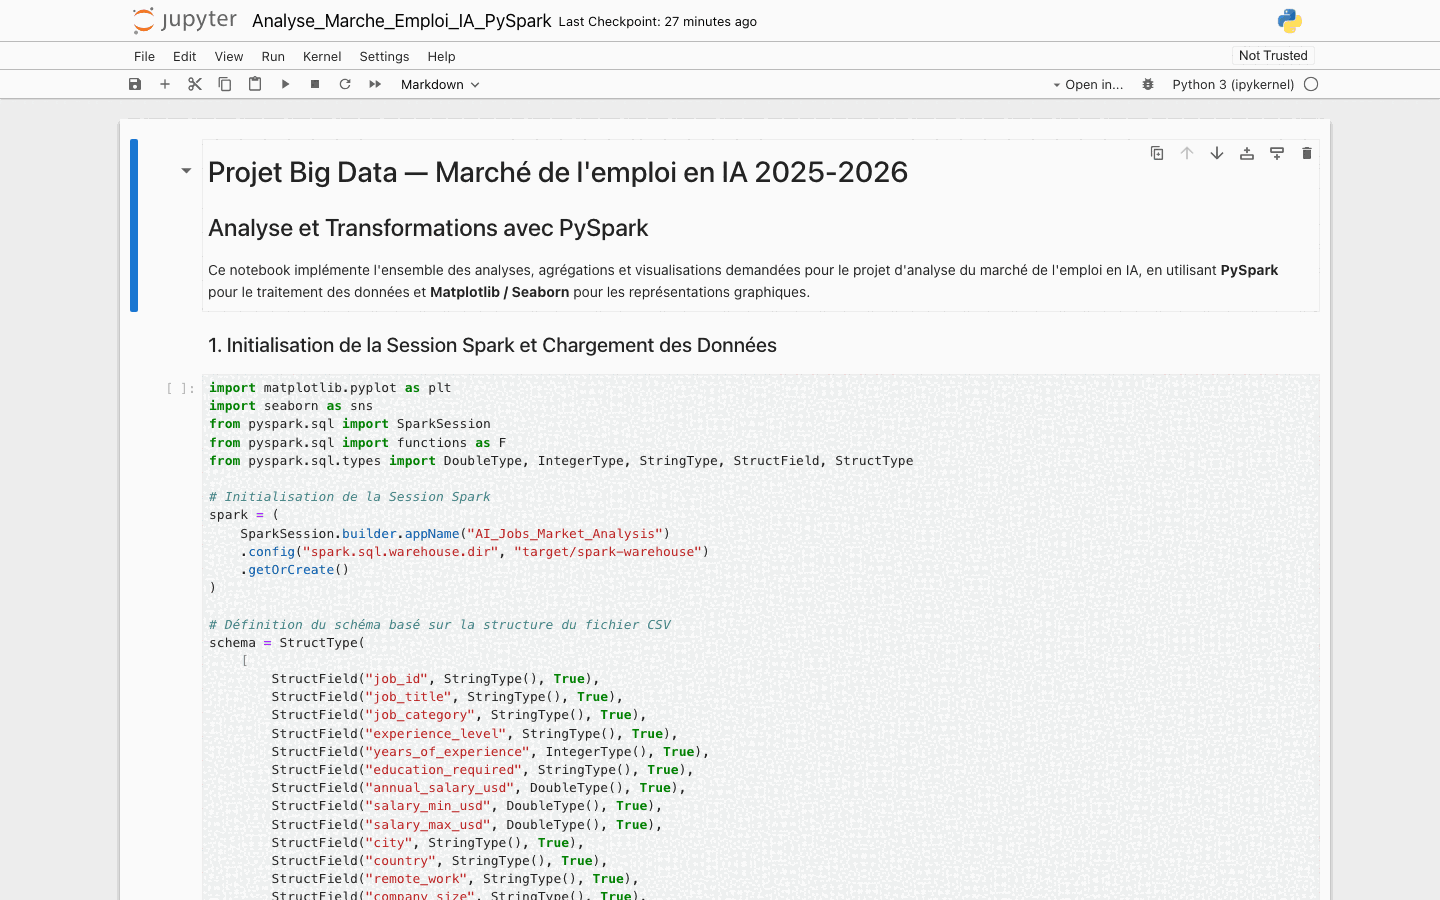
\includegraphics[width=0.75\linewidth]{figures/etape2_jupyter_notebook.png}
\caption{Environnement Jupyter/PySpark connecté à la stack, avec le
notebook du projet ouvert.}
\end{figure}

\section{Flux d'une requête type}

Le schéma d'architecture montre les composants et le flux de données au
niveau du pipeline. Le diagramme de séquence ci-dessous montre ce que
voit un utilisateur lors d'une requête interactive classique depuis
Jupyter/PySpark : chaque étape reste dans la stack, aucun accès direct au
CSV local n'est nécessaire.

\begin{figure}[h]
\centering
\resizebox{\linewidth}{!}{\begin{tikzpicture}[
  font=\small\sffamily,
  actor/.style={rectangle, rounded corners=3pt, fill=esieablue, text=white,
    minimum width=2.2cm, minimum height=0.75cm, align=center, draw=none},
  lifeline/.style={dashed, esieagray, line width=0.4pt},
  msg/.style={->, >=stealth, thick, esieagray},
  lbl/.style={font=\scriptsize\sffamily\color{esieagray}, align=center,
    fill=white, inner sep=1.5pt}
]
% Acteurs
\node[actor] (user) at (0,0) {Utilisateur};
\node[actor] (jupyter) at (3.8,0) {Jupyter/\\PySpark};
\node[actor] (hive) at (7.6,0) {Hive\\metastore};
\node[actor] (hdfs) at (11.4,0) {HDFS\\processed};

% Lifelines
\draw[lifeline] (user.south) -- (0,-5.5);
\draw[lifeline] (jupyter.south) -- (3.8,-5.5);
\draw[lifeline] (hive.south) -- (7.6,-5.5);
\draw[lifeline] (hdfs.south) -- (11.4,-5.5);

% Messages
\draw[msg] (0,-0.9) -- (3.8,-0.9) node[lbl, midway, above] {requête SQL / Spark SQL};
\draw[msg] (3.8,-1.7) -- (7.6,-1.7) node[lbl, midway, above] {demande de metadata};
\draw[msg] (7.6,-2.5) -- (3.8,-2.5) node[lbl, midway, above] {location Parquet};
\draw[msg] (3.8,-3.3) -- (11.4,-3.3) node[lbl, midway, above] {lecture des fichiers Parquet};
\draw[msg] (11.4,-4.1) -- (3.8,-4.1) node[lbl, midway, above] {DataFrame / résultats};
\draw[msg] (3.8,-4.9) -- (0,-4.9) node[lbl, midway, above] {tableau / visualisation};

% Zone d'activation Jupyter
\draw[fill=esieaoffwhite, draw=esieagray, rounded corners=2pt, line width=0.5pt]
  (3.5,-0.7) rectangle (4.1,-5.1);
\end{tikzpicture}
}
\caption{Flux d'une requête type : utilisateur $\to$ Jupyter/PySpark
  $\to$ Hive (métadonnées) $\to$ HDFS (fichiers Parquet) $\to$ retour
  des résultats sous forme de tableau ou de visualisation.}
\label{fig:sequence_requete}
\end{figure}

\section{Organisation raw / processed / output}

\begin{itemize}[leftmargin=1.5em]
  \item \texttt{/projet\_ia/raw} : CSV brut déposé par ingestion.
  \item \texttt{/projet\_ia/processed/\{offres,metiers,competences\}} :
    tables Parquet issues du pipeline ETL.
  \item \texttt{/projet\_ia/output} : réservé aux exports du dashboard
    et analyses finales.
\end{itemize}
